%% 
%% Copyright 2019-2020 Elsevier Ltd
%% 
%% This file is part of the 'CAS Bundle'.
%% --------------------------------------
%% 
%% It may be distributed under the conditions of the LaTeX Project Public
%% License, either version 1.2 of this license or (at your option) any
%% later version.  The latest version of this license is in
%%    http://www.latex-project.org/lppl.txt
%% and version 1.2 or later is part of all distributions of LaTeX
%% version 1999/12/01 or later.
%% 
%% The list of all files belonging to the 'CAS Bundle' is
%% given in the file `manifest.txt'.
%% 
%% Template article for cas-dc documentclass for 
%% double column output.

%\documentclass[a4paper,fleqn,longmktitle]{cas-dc}
\documentclass[a4paper,fleqn]{cas-dc}

%\usepackage[authoryear,longnamesfirst]{natbib}
%\usepackage[authoryear]{natbib}
\usepackage[numbers]{natbib}

%%%Author definitions
\def\tsc#1{\csdef{#1}{\textsc{\lowercase{#1}}\xspace}}
\tsc{WGM}
\tsc{QE}
\tsc{EP}
\tsc{PMS}
\tsc{BEC}
\tsc{DE}
%%%
% -------------------------------------------------------------------
% Pacotes para inserção de figuras e subfiguras
% \usepackage{subfig,epsfig,tikz,float}		            % Packages de figuras. 
\usepackage{graphicx}
\usepackage{caption}
\usepackage{subcaption}
\graphicspath{ {./figs/} }

% -------------------------------------------------------------------
% \usepackage{amssymb}
% -------------------------------------------------------------------
% Pacotes para inserção de tabelas
\usepackage{booktabs,multicol,multirow,tabularx,array}          % Packages para tabela
\usepackage{natbib}
\usepackage{pifont}
\usepackage{xcolor}
\usepackage{algpseudocode}
\usepackage{algorithm}
% -------------------------------------------------------------------
\PassOptionsToPackage{style=super,nolist}{glossaries}
\PassOptionsToPackage{acronym}{glossaries}
\PassOptionsToPackage{nonumberlist}{glossaries}
\usepackage{glossaries}
\newacronym{cnn}{CNN}{Convolutional Neural Network}
\newacronym{cv}{CV}{Computer Vision}
\newacronym{ca}{CA}{Conversational Agents}
\newacronym{cs}{CS}{Conversational Systems}
\newacronym{sr}{SR}{Speech Recognition}
\newacronym{nlp}{NLP}{Natural Language Processing}
\newacronym{ml}{ML}{Machine Learning}
\newacronym{nlu}{NLU}{Natural Language Understanding}
\newacronym{ai}{AI}{Artificial Inteligence}
\newacronym{er}{ER}{Named Entity Recognition}
\newacronym{sa}{SA}{Sentiment Analysis}
\newacronym{lsa}{LSA}{Latent Semantic Analysis}
\newacronym{svm}{SVM}{Support Vector Machine}
\newacronym{nn}{NN}{Neural Networks}
\newacronym{rnn}{RNN}{Recurrent Neural Network}
\newacronym{lstm}{LSTM}{Long Short-Term Memory}
\newacronym{bilstm}{BILSTM}{Bidirectional Long Short-Term Memory}
\newacronym{me}{ME}{Maximum Entropy}
\newacronym{bn}{BN}{Bayesian Network}
\newacronym{nb}{NB}{Naive Bayes}
\newacronym{knn}{KNN}{K-Nearest Neighbor}
\newacronym{dt}{DT}{Decision Tree}
\newacronym{pgwbi}{PGWBI}{Psychological General Well-Being Index}
\newacronym{dhs}{DHS}{Depression-Happiness Scale}
\newacronym{panas}{PANAS}{Positive Affect Negative Affect Scale}
\newacronym{ohq}{OHQ}{Oxford Happiness Questionnaire}
\newacronym{abs}{ABS}{Affect Balance Scale}
\newacronym{w_bq12}{W-BQ12}{Well-being Questionnaire}
\newacronym{esat}{ESAT}{Emotional State Assessment Tool}
\newacronym{gds}{GDS}{Geriatric Depression Scale}
\newacronym{gds_15}{GDS-15}{Geriatric Depression Scale-15}
\makeglossaries
% -------------------------------------------------------------------
\usepackage[utf8]{inputenc} % The default since 2018
\DeclareUnicodeCharacter{200B}{{\hskip 0pt}}
% -------------------------------------------------------------------
\begin{document}
\let\WriteBookmarks\relax
\def\floatpagepagefraction{1}
\def\textpagefraction{.001}
\shorttitle{EmoCare}
\shortauthors{Carla Mendes et~al.}

\title [mode = title]{EmoCare}                     

\credit{Conceptualization of this study, Methodology, Software}

\author[1]{Carla Mendes}[type=editor,
		%auid=000,bioid=1,
		linkedin='carla-mendes-5b3586233',
		orcid=0000-0001-7138-7124]
%\cormark[1]
%\fnmark[1]
\ead{carla.c.mendes@ipleiria.pt}

\address[1]{Computer Science and Communications Research Centre, School of Technology and Management, Polytechnic of Leiria, 2411-901 Leiria, Portugal}

\begin{abstract}
Abstract goes here.


\end{abstract}

%\begin{graphicalabstract}
%
\includegraphics{figs/grabs.pdf}
%\end{graphicalabstract}
%
%\begin{highlights}
%\item Research highlights item 1
%\item Research highlights item 2
%\item Research highlights item 3
%\end{highlights}

\begin{keywords}

\end{keywords}


\maketitle

\section{Introdution}
\label{introduction}

\section{Related work}
\label{relatedWork}

\section{Background and contextualization}
\label{backgroundContextualization}

This section aims to review existing literature regarding \gls{ca}, \gls{sa} and mood assessment questionnaires.

\subsection{Conversational agents}
\label{conversationalAgents}

Chatbots, referred to as \gls{ca} or \gls{cs}, are software applications created to imitate human-computer interactions  \cite{montenegro_survey_2019}.

\subsubsection{Classification methods}

Chatbots can be categorized based on various factors, including their goal, interaction mode, knowledge domain, and response-generation method \cite{hussain_survey_2019}.

\gls{cs} operate using different modes of interaction, namely based on text or speech. In the text-based mode, users communicate with the chatbot by typing their queries or statements, commonly through chat applications, messaging platforms, or web-based chat interfaces. The chatbot responds with text-based messages in return. On the other hand, speech-based chatbots enable users to interact with the chatbot using spoken language. These chatbots employ \gls{sr} technology to convert the user's voice input into text, which is then processed and analyzed to generate appropriate responses. Voice-based chatbots are typically found in voice assistants like Amazon Alexa, Google Assistant, or Apple Siri. They offer a convenient and hands-free method of interacting with the chatbot, enabling users to engage in natural conversations and perform tasks using voice commands. Additionally, chatbots can also adopt a multi-modal approach, allowing interaction through both text and speech \cite{montenegro_survey_2019}.

When considering their objective, chatbots are categorized as either task-oriented or non-task-oriented. Task-oriented chatbots are designed with a specific purpose, focusing on handling particular tasks and engaging in brief conversations, typically within a limited domain. Conversely, non-task-oriented chatbots specialize in emulating conversations with individuals and participating in casual chitchat primarily for entertainment. As a result, they operate in open domains, facilitating more diverse and unrestricted conversations \cite{hussain_survey_2019}.

In terms of response generation methods, chatbots are also classified based on the techniques and algorithms used to generate suitable and meaningful responses to user queries or inputs. These methods can be categorized as follows:

\begin{itemize}
	\item \textbf{Rule-based}: rely on a predefined set of rules and patterns to generate responses. Human experts typically create these rules and program them into the chatbot system. The \gls{ca} then matches user inputs with specific patterns or keywords and retrieves corresponding responses. Rule-based systems work well for simple and structured conversations but may struggle with complex or unpredictable queries.
	\item \textbf{Retrieval-based}: use \gls{ml} techniques to select the most appropriate response based on the user's input from a large dataset of predefined responses. Retrieval-based systems may struggle with creative responses, however provide contextually relevant responses.
	\item \textbf{Template-based}:  use pre-built response templates that are filled with relevant information based on user inputs. These templates contain placeholders for dynamic content such as names, dates, or specific details. The chatbot captures the intents of the user's input and selects an appropriate template to generate a response. Template-based systems may lack flexibility and creativity in generating unique responses but are relatively simple to implement.
	\item \textbf{Generative-based}: rely on advanced \gls{nlp} techniques and \gls{ml} models to create responses from scratch, namely sequence-to-sequence models or transformers. These models are trained on large datasets and learn the patterns and structures of human language. Generative models are more versatile in handling diverse user inputs. However, they can be more computationally intensive and require significant computational resources for training and inference.
	\item \textbf{Hybrid Approach} - combine multiple methods mentioned above to leverage the strengths of each approach.
\end{itemize}

Lastly, in the knowledge domain dimension, chatbots possess specialized knowledge and capabilities tailored to serve specific purposes within a limited scope. They possess knowledge and capabilities customized to fulfill specific objectives or offer assistance within a restricted topic. These chatbots undergo training and programming to comprehend and address inquiries regarding a specific domain. For instance, a chatbot tailored to a particular subject can aid in customer support for an e-commerce platform, provide medical advice in the healthcare sector, or offer travel recommendations within the tourism industry. On the other hand, open-domain chatbots engage in conversations spanning a broad spectrum of topics, free from confinement to any specific domain. They aim to emulate human-like interactions, delivering casual conversation, entertainment, or general information across various subjects \cite{mohamad_2021}.

\subsubsection{General Architecture}

A robust \gls{ca} system will possess several key components, represented in Figure \ref{fig:ConversationalAgentGeneralArchitecture}.

\begin{figure}[htbp]
	\centering
	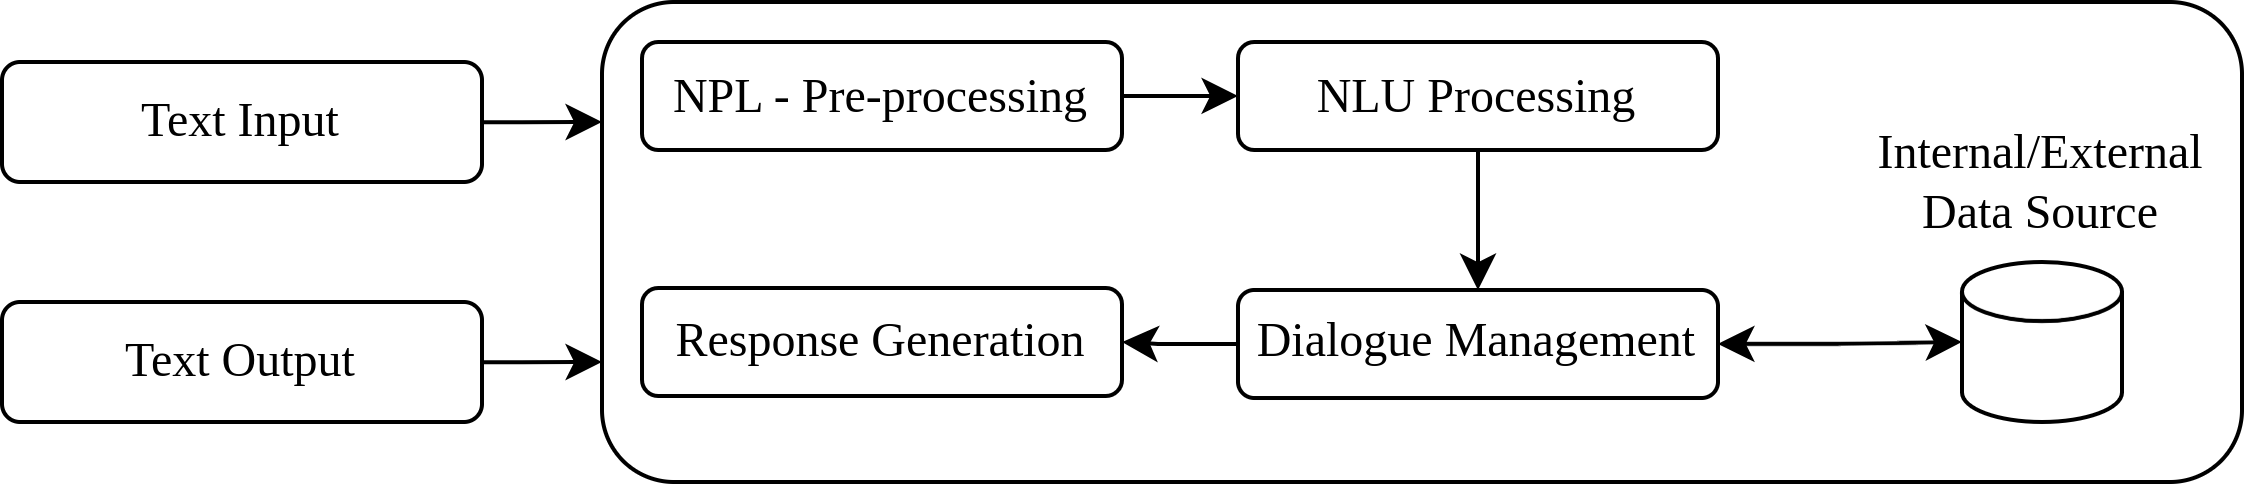
\includegraphics[width=\linewidth]{figs/ConversationalAgentGeneralArchitecture.png}
	\caption{Conversational agents general architecture.}
	\label{fig:ConversationalAgentGeneralArchitecture}
\end{figure}

During the \gls{nlp} phase, the user's request undergoes various techniques, including tokenization, lemmatization, and stemming. These techniques help extract structured data from the request, which is then passed on to the subsequent component, known as the \gls{nlu} module, responsible for analyzing each incoming user request using various strategies, namely, parsing the request to understand the user's intention and the associated details. The dialogue management module focuses on keeping track of the dialogue context and defining the following actions to perform by analyzing the input request that has been transformed into understandable structured data by the \gls{ca} system. The data sources serve as repositories for information and data utilized by the dialogue manager. These sources can be either internal or external. Internally, chatbots can access data from templates or rules to understand user requests and generate appropriate responses. Moreover, \gls{ca} can also build their databases from scratch or leverage existing databases that align with their domain and functionality. In contrast, external data sources can be accessed through third-party services like Web APIs, which provide the necessary information. The response generator module plays a crucial role in generating an appropriate response from a pool of potential options after executing an action. This component utilizes the approaches mentioned earlier to generate the most suitable response for the given context. \cite{rizou_multilingual_2022, mohamad_suhaili_service_2021}

\subsubsection{Tools}

Rasa \cite{rasa} is an open-source dialogue framework for building conversational \gls{ai} applications. It uses \gls{nlp} techniques and dialogue management to enable interactive and context-aware conversations. Rasa consists of two main components: the \gls{nlu} module for processing user inputs and extracting intents and entities, and the Dialogue Management module for handling conversation flow and decision-making. It supports personalized dialogue policies, provides tools for training and evaluation, and integrates with different channels and platforms. Rasa supports both text-based and voice-based interactions, making it versatile for various applications.

Amazon Lex \cite{aws} is a service provided by Amazon Web Services that allows developers to build, test, and deploy \gls{ca} powered by \gls{ai}. It is designed to create interactive chatbots and virtual assistants that can understand natural language inputs and provide appropriate responses. Amazon Lex leverages advanced natural language models and \gls{ml} algorithms to enable accurate understanding and interpretation of user inputs. It supports both text and speech inputs and outputs, making it suitable for various applications. With Amazon Lex, developers can easily integrate \gls{ca} into their applications or platforms, enabling more intuitive and engaging user experiences.

Dialogflow \cite{dialogflow} is a \gls{nlu} platform developed by Google. It provides tools and capabilities for building \gls{ca}, chatbots, and virtual assistants. With Dialogflow, developers can create, manage, and deploy \gls{ca} across multiple platforms and systems. It supports both text and speech inputs and outputs, allowing users to interact with the \gls{ca} through various channels such as messaging platforms, voice assistants, and websites. This platform utilizes advanced \gls{ml} algorithms to understand and interpret user inputs, extracting important information such as intents (the user's intention) and entities (specific pieces of information). It offers a range of pre-built \gls{nlu} components and features, including \gls{er} and \gls{sa}. Additionally, Dialogflow provides a visual interface for designing conversation flows, managing dialogues, and defining responses.

OpenDial \cite{opendial} is an open-source Java-based toolkit used for building and evaluating speech-based \gls{ca}. It provides a framework and set of tools that enable developers to create interactive dialogue systems capable of engaging in natural language conversations. Furthermore, the toolkit offers a range of features and functionalities for building \gls{ca}. It provides modules for \gls{nlu}, dialogue management, and speech synthesis. OpenDial allows developers to define dialogue policies and strategies to guide the system's behaviour and response generation. It also includes components for handling user input, managing context, and generating appropriate spoken responses. Overall, OpenDial emphasizes modularity and extensibility, enabling developers to customize and adapt the toolkit according to their specific requirements. 

Botpress \cite{botpress} is an open-source platform that enables developers to build, deploy, and manage chatbots and virtual assistants. It provides a visual interface for designing conversational flows and supports both text-based and voice-based interactions. Botpress is written in JavaScript and can be deployed on various platforms. One of the key features of Botpress is its visual flow builder, which allows developers to create complex conversational flows using a drag-and-drop interface. This makes it easy to design the dialogue flow of the chatbot and define the interactions between the user and the bot. Botpress also offers built-in \gls{nlu} capabilities, allowing developers to train the chatbot to understand user intents and extract entities from user inputs.

ChatterBot \cite{chatterbot} is an open-source Python library that facilitates the development of chatbots. The primary focus of ChatterBot is to generate responses based on pre-defined conversational patterns. It uses a machine learning algorithm called \gls{lsa} to train a language model on a given corpus of text data and  then generate appropriate responses based on the patterns it has learned. ChatterBot supports the use of multiple languages and provides various pre-trained language models that can be used out of the box. Additionally, it enables developers to customize the chatbot's behaviour by defining rules, selecting appropriate responses, and handling specific cases. One of the notable features of ChatterBot is its ability to learn and improve over time. It employs a technique called "conversational context" to maintain the history of the conversation and generate contextually relevant responses. 

\subsection{Sentiment Analysis}

\gls{sa}, a subfield of \gls{nlp}, aims to derive the sentiments expressed in a piece of text based on its content, which can be conducted at different levels: Document Level, Sentence Level, Phrase Level, and Aspect Level  \cite{kaur_survey_2017, wankhade_survey_2022}.

Document-level \gls{sa} involves assessing the sentiment of an entire document and assigning a single polarity to it. Classification methods, both supervised and unsupervised, can be employed at this level to determine the sentiment conveyed in the document \cite{wankhade_survey_2022}.

At the Sentence Level, each sentence is analyzed and classified into a polarity sentiment. This approach more valuable when a document contains a diverse range of sentiments. By independently determining the polarity of each sentence, either using methodologies similar to document-level analysis or with more extensive training data and processing resources, the overall sentiment of the document can be aggregated or analyzed sentence by sentence  \cite{wankhade_survey_2022}.

The Phrase Level of \gls{sa} focuses on mining opinion words and sentiments at the phrase level. While document-level analysis broadly categorizes the entire document as either positive or negative, sentence-level analysis proves more advantageous because documents often contain both positive and negative statements. At this level, individual words become the fundamental units of language, and their polarity is intrinsically tied to the subjectivity of the sentences or documents in which they appear \cite{wankhade_survey_2022}.

Lastly, Aspect Level delves even deeper, as it is performed on specific aspects within a sentence. Since a sentence may contain multiple aspects, this approach pays close attention to all aspects present and assigns polarity to each one. An aggregate sentiment is then calculated for the entire sentence, considering the sentiments of all its aspects.

To conduct \gls{sa}, several main steps are followed, including data collection, feature selection, feature extraction, and the use of word embeddings. These steps aid in gathering relevant data, choosing essential features, extracting meaningful patterns, and representing words in a numerical format suitable for analysis  \cite{kaur_survey_2017}.

\subsubsection{Approaches}

There are three main approaches commonly used for \gls{sa}: the Lexicon Based Approach, the \gls{ml} Approach, and the Hybrid Approach \cite{wankhade_survey_2022, kaur_survey_2017}.

Lexicons consist of tokens, with each token having a predefined score that indicates the neutral, positive, or negative nature of the text. The lexicon-based method is highly suitable for conducting \gls{sa} at both the sentence and feature levels. Initially, the document is divided into tokens of individual words, and then the polarity of each token is calculated and aggregated. There are primarily two approaches used in Lexicon Based Approaches: the Corpus Based Approach and the Dictionary based approach \cite{wankhade_survey_2022}.

The Corpus-based approach utilizes semantic and syntactic patterns to determine the emotion of a sentence. It begins with a predefined set of sentiment terms and their orientations, then explores syntactic or similar patterns within a vast corpus to identify sentiment tokens and their orientations. This method is specific to the situation and requires a substantial amount of labeled data for training. Within the corpus-based approach, there are two types of approaches: the Statistical Approach and the Semantic Approach \cite{wankhade_survey_2022, kaur_survey_2017}.

On the other hand, the Dictionary-Based Approach commences by manually collecting a set of opinion words to form a seed list. Next, dictionaries and thesauruses are consulted to find synonyms and antonyms of these words, which are then added to the seed list. This process continues until no new words are discovered. However, a drawback of this approach is the challenge of finding context or domain-oriented opinion words \cite{wankhade_survey_2022, kaur_survey_2017}.

There are two primary in \gls{ml} approaches: Supervised \gls{ml} and Lexicon-based unsupervised learning \cite{wankhade_survey_2022}.

In Lexicon-based unsupervised strategies, knowledge bases, ontologies, databases, and lexicons containing specific and detailed information for \gls{sa} are utilized. On the other hand, supervised learning methods are more widely used due to their high accuracy. These algorithms require training on a labeled dataset before they can be applied to real data. Features are extracted from the text data during the training process \cite{kaur_survey_2017}.

The \gls{ml} technique uses syntactic or linguistic factors to classify sentiment and constitute a text classification problem. Therefore, the model associates features of the underlying record with class labels and predicts the label for unknown instances \cite{kaur_survey_2017}. Commonly used \gls{ml} algorithms include:

\begin{itemize}
	\item \textbf{\gls{dt} classifier}
	\item \textbf{Linear classifier} - e.g. \gls{svm} and Neural Networks such as \gls{rnn}, \gls{cnn}, \gls{lstm} and \gls{bilstm}, Transformers
	\item \textbf{Rule-based classifier} 
	\item \textbf{Probabilistic classifiers} - e.g. Multinomial \gls{nb}, \gls{me} and \gls{bn}
	\item \textbf{\gls{knn}}
\end{itemize}

The hybrid approach combines \gls{ml} and lexicon-based techniques. It refers to the integration of both methods to enhance the accuracy and effectiveness of the systems. By leveraging the strengths of both approaches, the hybrid method can provide more comprehensive insights into the sentiment expressed in the text  \cite{wankhade_survey_2022}.

\subsubsection{Datasets}

There are diverse datasets used to train \gls{sa} algorithms, some of which include: SemEval 2007 task 14 corpus, ISEAR, SentiWordNet, IMDB, SST and NRC.

The SemEval 2007 task 14 corpus \cite{strapparava_learning_2008} consists of emotional newspaper headlines from reputable sources like the New York Times, CNN, BBC, or Google News. This corpus allows training models for emotions such as anger, disgust, fear, joy, sadness, and surprise.

ISEAR \cite{ISEAR} is a dataset comprising psychological data from a survey conducted in 1990. In this dataset, 3,000 subjects described situations where they felt various emotions, including joy, sadness, fear, anger, disgust, shame, or guilt.

The SentiWordNet dataset \cite{baccianella_sentiwordnet_2010} is a publicly available dataset that automatically labels synsets in the WordNet dataset based on their degree of positivity, negativity, and neutrality.

The IMDB Movie Reviews dataset \cite{IMDB} is publicly available and contains around 50,000 movie reviews, labeled as either positive or negative.

SST \cite{SST} is a sentiment analysis dataset from Stanford, containing 10,662 movie sentences from Rotten Tomatoes, labeled with corresponding emotions, ranging from "very negative" to "very positive."

NRC \cite{SaifmohammadLexicons} is a comprehensive emotion Lexicon dataset, containing more than 14,000 words annotated with sentiment (positive or negative) and various emotions, such as anger, anticipation, disgust, fear, joy, sadness, surprise, and trust.

\subsection{Mood Assessment Questionnaires}

% tomorrow morning: https://www.notion.so/carla-mendes/ERNUI-33d6da683fae4ed494e9a928b7a16a50

The \gls{pgwbi} \cite{grossi_psychological_2014} is a questionnaire to measure subjective psychological well-being, assessing emotional states that reflect a sense of well-being or distress. It consists of 22 standardized items (or 6 for the short form), producing a single well-being score. It includes subscales for anxiety, depression, positive well-being, self-control, general health, and vitality. The original \gls{pgwbi} has 22 self-administered items, rated on a 6-point scale, covering six HRQoL domains: anxiety, depression, positive well-being, self-control, general health, and vitality. Each item scores from 0 to 5, referring to the last 4 weeks. The domains have 3 to 5 items each. All domain scores contribute to a global summary score, with a theoretical maximum of 110 points. The short form, containing six items, explains over 92\% of the variance of the full questionnaire.

The \gls{dhs} \cite{mcgreal_depression_happiness_1993, joseph_rapid_SDHS} is a psychometric tool utilized to evaluate an individual's levels of depression and happiness, to measure their emotional well-being and mood. The questionnaire consists of 25 items, 12 assessing happiness, and the remaining 13 focus on depression. However, there is also a short version comprising 6 items, where 3 measure happiness and the other 3 measure depression. Respondents are asked to reflect on their feelings over the past seven days and rate each item on a 4-point scale: "never" (0), "rarely" (1), "sometimes" (2), and "often" (3). The positive items are directly scored, while the negative ones are reversed-scored. The scores on the 25-item scale range from 0 to 75, with higher scores indicating a greater sense of happiness and lower scores suggesting lower levels of depression. 

The \gls{panas} \cite{tran_positive_2013} is a widely used scale for assessing mood or emotions. It consists of 20 items, with 10 items dedicated to measuring positive affect (e.g., excited, inspired) and 10 items for negative affect (e.g. upset, afraid). Respondents rate each item on a five-point Likert Scale, indicating the extent to which they have experienced the particular effect within a specified time frame. The PANAS is designed to gauge affect in various contexts, such as the present moment, the past day, week, year, or overall (on average). As a result, the scale measures current emotional state, enduring or trait-based emotions, fluctuations in emotions over a specific period, or emotional responses to specific events.

The \gls{ohq} \cite{hills_oxford_2002} is a questionnaire designed to assess an individual's happiness, covering various dimensions such as positive emotions, life satisfaction, sense of purpose, and overall well-being. The \gls{ohq} consists of 29 items, each presented as a single statement, which respondents rate on a uniform six-point Likert scale. Researchers used discriminant analysis to create a shorter version of the \gls{ohq} and identified eight key items. The final \gls{ohq} score is calculated by summing the responses to positive items and reverse-scored negative items and then dividing by the total number of items (29). This calculation results in scores ranging from 1 to 6, reflecting the participants ' level of happiness based on their responses to the questionnaire, with lower values indicating sadness and higher values of positivity.

Affectometer 2 \cite{kammann_affectometer_1983} is a 40-item self-report scale designed to measure general happiness or well-being by assessing the balance of positive and negative emotions experienced in recent times. It takes approximately 5 minutes to complete. The questionnaire contains separate items for measuring both positive and negative affect. Participants rate the extent to which they have experienced each emotion within a specific time frame, such as the past week or month. They provide their responses using a Likert-type scale, indicating their agreement or frequency of experiencing each emotion. The total score on the Affectometer 2 represents the difference between the positive and negative affect, reflecting an individual's overall emotional balance. In the development of the scale, the authors categorized the items into 10 mnemonic groups, referred to as "qualities of happiness." They aimed to include four items for each category, with one each from positive sentences, negative sentences, positive adjectives, and negative adjectives. To complete the 40-item matrix, the researchers retrieved four items from the original item pool and created and validated six new ones.

The \gls{abs} \cite{glatzer_affect_2014} is a comprehensive measure used to assess specific aspects of quality of life in both national and international contexts. It consists of a 10-item Subjective Well-Being Scale, with five questions focused on positive feelings and five statements related to negative feelings. Participants respond to the questions without gradation, indicating either a "yes" or "no" to each item. This format allows for the summation of responses, resulting in scores ranging from 0 to 5 for both the positive and negative affect subscales. Higher scores on each subscale indicate greater levels of positive and negative affect, respectively. Researchers sometimes use the final score, which is the difference between the positive affect and negative affect scores, as an indicator of overall happiness.

\gls{w_bq12} \cite{mitchell_psychometric_2001} is a self-report psychometric tool used to assess an individual's subjective well-being and overall quality of life. It is designed to measure various dimensions of well-being, including emotional, psychological, and social aspects. The W-BQ12 consists of 12 items, each addressing different aspects of well-being. Participants are asked to rate the extent to which they agree or disagree with each statement based on their feelings and experiences. Responses are typically measured on a Likert-type scale, where participants indicate their level of agreement or disagreement or the frequency of experiencing certain feelings or thoughts. The questionnaire covers a wide range of well-being dimensions, including positive affect, life satisfaction, self-esteem, and social relationships. By analyzing the responses, researchers and practitioners can gain insights into an individual's overall sense of well-being and emotional health.

The \gls{esat} \cite{yaden_emotional_2022} is a measure of emotional well-being based on a two-dimensional model of affect (positive and negative emotion) and a six-dimensional model (cheerfulness, vitality, serenity, sadness, lethargy, and stress) derived from a philosophical theory of affect. The tool was developed through a series of studies, resulting in an 18-item questionnaire that offers a more detailed understanding of positive and negative affect, providing a versatile and cross-culturally sensitive assessment of emotions. 

The \gls{gds} \cite{yesavage_development_1982} is a short, self-administered questionnaire designed to assess depressive symptoms in older adults. It is specifically developed for use with individuals aged 65 years and older, although it can also be used with younger adults in certain circumstances. The \gls{gds} is a widely used screening tool to identify potential depression in older adults, particularly in clinical settings, research studies, and geriatric assessments, and possesses numerous versions. One of which is the \gls{gds_15} a questionnaire with yes-or-no questions where participants are asked to respond based on how they felt over the past week.  Of the 15 items, 10 indicated the presence of depression when answered positively, while the rest (question numbers 1, 5, 7, 11, 13) indicated depression when answered negatively. Scores of 0-4 are considered normal, depending on age, education, and complaints; 5-8 indicate mild depression; 9-11 indicate moderate depression; and 12-15 indicate severe depression. 

\section{Architecture}
\label{architecture}

\section{Proposed solution and implementation}
\label{proposedSolution}

\section{Conclusion}
\label{conclusion}
\printcredits

%% Loading bibliography style file
%\bibliographystyle{model1-num-names}
%\bibliographystyle{cas-model2-names}
\bibliographystyle{unsrt} % Estilo de Bibliografia
% Loading bibliography database
\bibliography{cas-refs}


%\vskip3pt

\end{document}
